% motivation.tex
% Section 1: Why Programming Education Must Change in the LLM Era

%%%%%%%%%%%%%%%%%%%%
\section{Motivation: Why Programming Education Must Change}
%%%%%%%%%%%%%%%%%%%%

%%%%%%%%%%%%%%%%%%%%
\begin{frame}{The LLM Revolution in Programming}
  \begin{center}
    \textbf{Large Language Models have fundamentally changed how we write code.}
  \end{center}
  
  \vspace{0.5cm}
  
  \begin{columns}[T]
    \begin{column}{0.48\textwidth}
      \textbf{\teal{What LLMs Excel At:}}
      \begin{itemize}
        \item Syntax generation
        \item API lookups
        \item Boilerplate code
        \item Pattern matching
        \item Documentation retrieval
      \end{itemize}
    \end{column}
    \begin{column}{0.48\textwidth}
      \textbf{\red{What LLMs Struggle With:}}
      \begin{itemize}
        \item Deep semantic reasoning
        \item Undefined behavior analysis
        \item Memory model understanding
        \item Design trade-off evaluation
        \item Historical context
      \end{itemize}
    \end{column}
  \end{columns}
  
  % Speaker note: Emphasize that LLMs shift the bottleneck from syntax recall to conceptual reasoning
\end{frame}
%%%%%%%%%%%%%%%%%%%%

%%%%%%%%%%%%%%%%%%%%
\begin{frame}{The Shifting Bottleneck}
  \begin{center}
    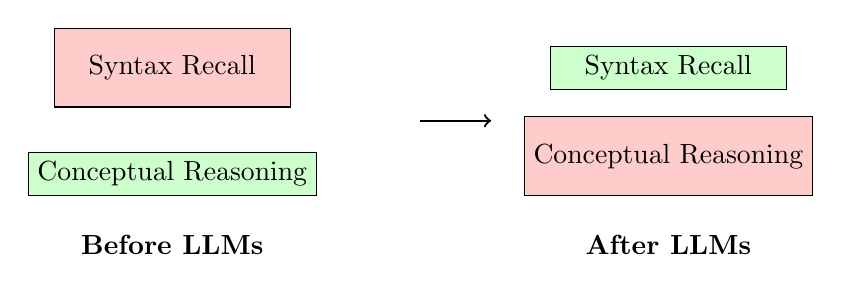
\begin{tikzpicture}[scale=0.9]
      % Before LLMs
      \node[draw, rectangle, fill=red!20, minimum width=3cm, minimum height=1cm] at (-3.5, 2) {Syntax Recall};
      \node[draw, rectangle, fill=green!20, minimum width=3cm, minimum height=0.5cm] at (-3.5, 0.5) {Conceptual Reasoning};
      \node at (-3.5, -0.5) {\textbf{Before LLMs}};
      
      % After LLMs
      \node[draw, rectangle, fill=green!20, minimum width=3cm, minimum height=0.5cm] at (3.5, 2) {Syntax Recall};
      \node[draw, rectangle, fill=red!20, minimum width=3cm, minimum height=1cm] at (3.5, 0.75) {Conceptual Reasoning};
      \node at (3.5, -0.5) {\textbf{After LLMs}};
      
      % Arrow
      \draw[->, thick] (0, 1.25) -- (1, 1.25);
    \end{tikzpicture}
  \end{center}
  
  \vspace{0.3cm}
  
  \begin{block}{Key Insight}
    The bottleneck has shifted from \textbf{remembering syntax} to \textbf{understanding why code works} (or doesn't).
  \end{block}
  
  % Speaker note: Reference Perlis's Epigram #7: "It is easier to write an incorrect program than understand a correct one."
\end{frame}
%%%%%%%%%%%%%%%%%%%%

%%%%%%%%%%%%%%%%%%%%
\begin{frame}[fragile]{The Danger: LLM Hallucinated Correctness}
  \textbf{Example: LLM-generated C code with hidden undefined behavior}
  
  \begin{block}{Seemingly Correct Code}
\begin{verbatim}
int *get_array_element(int *arr, size_t index) {
    return &arr[index];  // No bounds checking!
}

int sum_array(int *a, int *b, int n) {
    int sum = 0;
    for (int i = 0; i < n; i++)
        sum += a[i] + b[i];  // Aliasing issue!
    return sum;
}
\end{verbatim}
  \end{block}
  
  \vspace{0.2cm}
  \red{\textbf{Problems:}} Buffer overflow, pointer aliasing violations (C99 Rationale, \S6.5)
  
  % Speaker note: LLMs generate syntactically correct code that may invoke undefined behavior
\end{frame}
%%%%%%%%%%%%%%%%%%%%

%%%%%%%%%%%%%%%%%%%%
\begin{frame}{Why Understanding Design Rationale Matters}
  \begin{quote}
    ``C is a language that trusts the programmer.'' \\
    \hfill --- \textit{Dennis Ritchie, The Development of the C Language}
  \end{quote}
  
  \vspace{0.5cm}
  
  \textbf{Students must understand:}
  \begin{enumerate}
    \item \textbf{Why} C has undefined behavior (optimization freedom)
    \item \textbf{Why} Java has checked exceptions (explicit error handling)
    \item \textbf{Why} memory alignment exists (hardware constraints)
    \item \textbf{How} design choices affect real-world code
  \end{enumerate}
  
  \vspace{0.3cm}
  
  \begin{alertblock}{Teaching Implication}
    LLMs cannot teach \textit{why}---only instructors can provide historical and philosophical context.
  \end{alertblock}
  
  % Speaker note: Reference "The Development of the C Language" by Ritchie
\end{frame}
%%%%%%%%%%%%%%%%%%%%

%%%%%%%%%%%%%%%%%%%%
\begin{frame}{Execution Model Literacy Remains Critical}
  \begin{columns}[T]
    \begin{column}{0.55\textwidth}
      \textbf{What Students Must Understand:}
      \begin{itemize}
        \item C's abstract machine model
        \item Memory layout (stack, heap, data segments)
        \item Object lifetime and storage duration
        \item Sequence points and side effects
        \item The ``as-if'' rule
      \end{itemize}
    \end{column}
    \begin{column}{0.43\textwidth}
      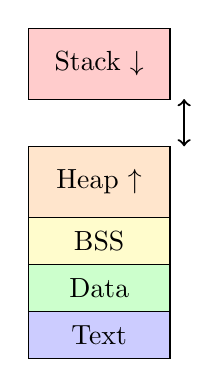
\begin{tikzpicture}[scale=0.6]
        \draw[fill=blue!20] (0,0) rectangle (3,1);
        \node at (1.5,0.5) {Text};
        \draw[fill=green!20] (0,1) rectangle (3,2);
        \node at (1.5,1.5) {Data};
        \draw[fill=yellow!20] (0,2) rectangle (3,3);
        \node at (1.5,2.5) {BSS};
        \draw[fill=orange!20] (0,3) rectangle (3,4.5);
        \node at (1.5,3.75) {Heap $\uparrow$};
        \draw[fill=red!20] (0,5.5) rectangle (3,7);
        \node at (1.5,6.25) {Stack $\downarrow$};
        \draw[<->, thick] (3.3, 4.5) -- (3.3, 5.5);
      \end{tikzpicture}
    \end{column}
  \end{columns}
  
  \vspace{0.3cm}
  
  \begin{block}{Reference: ISO C23 \S5.1.2.3}
    ``The semantic descriptions in this document describe the behavior of an abstract machine...''
  \end{block}
  
  % Speaker note: LLMs cannot reason about execution models without explicit training
\end{frame}
%%%%%%%%%%%%%%%%%%%%
